\documentclass{article}
\usepackage[utf8]{inputenc}
\usepackage[english]{babel}
\usepackage{algorithm}
\usepackage{algorithmicx}
\usepackage{listings}
\usepackage{graphicx}
\usepackage{vmargin}
\usepackage[noend]{algpseudocode}
\usepackage{listings}
\usepackage{color}
\usepackage[dvipsnames]{xcolor}
\usepackage{esvect}
\usepackage[spanish]{babel}
\usepackage[latin1]{inputenc}
\usepackage[usenames]{color}
\definecolor{backgroundColour}{rgb}{0.95,0.95,0.92}
\definecolor{mGreen}{rgb}{0,0.6,0}
\definecolor{mPurple}{rgb}{0.58,0,0.82}
\usepackage{hyperref}

\lstset{ 
	language=Matlab,                		
%	basicstyle=10pt,       			
	numbers=left,                  		
	numberstyle=\footnotesize,      		
	stepnumber=1,                   		
	numbersep=5pt,                  	
	backgroundcolor=\color{backgroundColour},
	commentstyle=\color{mGreen},
	keywordstyle=\color{blue},
	stringstyle=\color{mPurple},
	showspaces=false,               		
	showstringspaces=false,         		
	showtabs=false,                 			
%	tabsize=2,                			
%	captionpos=b,                   		
	breaklines=true,                			
	breakatwhitespace=false,        		
	escapeinside={\%*}{*)}          	
}


\usepackage{enumitem}

\setmargins{2.0cm}      % margen izquierdo
{1cm}                   % margen superior
{17cm}                  % anchura del texto
{23.42cm}               % altura del texto
{0cm}                   % altura de los encabezados
{1cm}                   % espacio entre el texto y los encabezados
{0cm}                   % altura del pie de página
{1cm}                   % espacio entre el texto y el pie de página


\title{
    Universidad Nacional de San Agustín 
    \\
    \large Escuela de Ingeniería de Sistemas
    \\
    \rule{100mm}{0.1mm}
    \\
    \huge Práctica 6
    \\
    \large Física Computacional

    \\
    \rule{100mm}{0.5mm}
    }
\author{Carlos Alberto Mestas Escarcena}
\date{Junio 2020}

\begin{document}

\maketitle
El desarrollo de este informe se puede encontrar en el repositorio de \textcolor{blue}{
    \href{https://github.com/CarlosMestas/FC---Pr-ctica-6}{GitHub}}.
\section{Ejercicio 1}

\begin{lstlisting} [frame=single]
clear; clf; hold off; n=0; h=0.001;
% Constantes del Sistema
k=0.1; m=0.2; c=0.0; F0=0.0; w=0.0;
% Condiciones Iniciales
t=0; x=2; vx=0; tfin=100; ax=-k*x/m-c*vx/m+F0/m*cos(w*t);
% Inicio de la Simulacion
pt(1)=t; pv(1)=vx; px(1)=x; pa(1)=ax;
pU(1) = 0.5 * k * x ^ 2;
pK(1) = 0.5 * m * vx ^ 2;
pE(1) = pU(1) + pK(1);
for t=0:h:tfin
    n  = n+1;
    ax =-k*x/m-c*vx/m+F0/m*cos(w*t);
    vx = vx + ax*h;
    x  = x  + vx*h;
    U = 0.5 * k * x .^ 2;
    K = 0.5 * m * vx .^ 2;
    E = U + K;
    pt(n+1)=t;
    px(n+1)=x;
    pv(n+1)=vx;
    pa(n+1)=ax;
    pU(n+1)=U;
    pK(n+1)=K;
    pE(n+1)=E;
end

% subplot(2,2,1), plot(pt,pa); grid on;
% xlabel('tiempo (s)');
% ylabel('Aceleracion (m/s^2)')
% subplot(2,2,2), plot(pt,pv); grid on;
% xlabel('tiempo (s)');
% ylabel('Velocidad (m/s)')
% subplot(2,2,3), plot(pt,px); grid on;
% xlabel('tiempo (s)');
% ylabel('Desplazamiento (m)')
% subplot(2,2,4), plot(px,pv); grid on;
% xlabel('Desplazamiento (m)');
% ylabel('Velocidad (m/s)')
% grid on;

% plot(px,pU,'DisplayName','Energía elástica')
% hold on
% plot(px,pK,'DisplayName','Energía cinética')
% plot(px,pE,'DisplayName','Energia total')
% grid on;
% legend

% plot3(px,pv,pt)
% grid on;
\end{lstlisting}

\begin{figure}[H]
\centering
    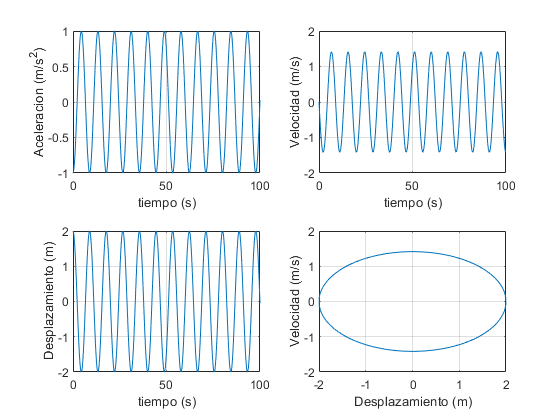
\includegraphics[width=1\textwidth]{images/001A.png}
    \caption{$x-t$, $v-t$, $a-t $~y $v-x$}
\end{figure}

\newpage
\clearpage

\begin{figure}[H]
\centering
    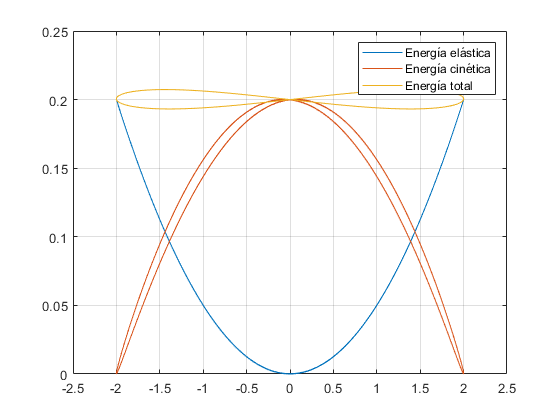
\includegraphics[width=0.5\textwidth]{images/001B.png}
    \caption{$h=0.1$}
\end{figure}

\begin{figure}[H]
\centering
    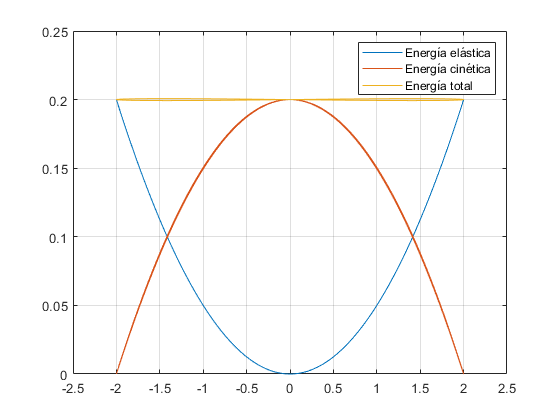
\includegraphics[width=0.5\textwidth]{images/001B2.png}
    \caption{$h=0.01$}
\end{figure}

\begin{figure}[H]
\centering
    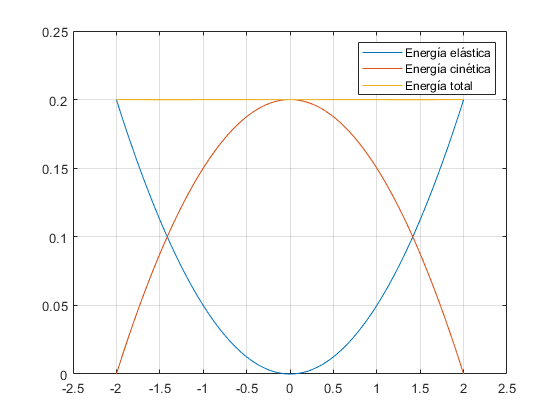
\includegraphics[width=0.5\textwidth]{images/001B3.png}
    \caption{$h=0.001$}
\end{figure}

\clearpage
\newpage

\begin{figure}[H]
\centering
    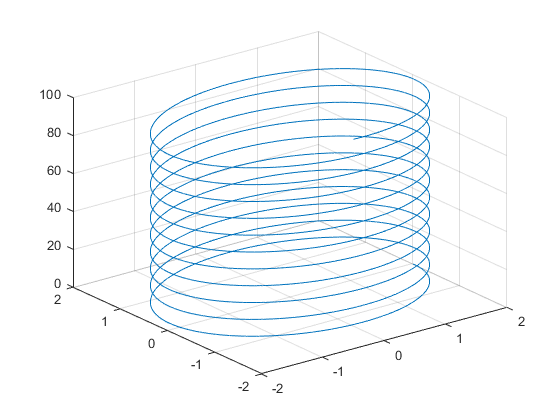
\includegraphics[width=0.7\textwidth]{images/001C.png}
    \caption{$v-x-t$}
\end{figure}

\section{Ejercicio 2}

\begin{lstlisting} [frame=single]
clear; clf; hold off; n=0; h=0.001;
% Constantes del Sistema
k=0.1; m=0.2; c=0.05; F0=0.0; w=0.0;
% Condiciones Iniciales
t=0; x=0; vx=-2; tfin=100; ax=-k*x/m-c*vx/m+F0/m*cos(w*t);
% Inicio de la Simulacion
pt(1)=t; pv(1)=vx; px(1)=x; pa(1)=ax;
pU(1) = 0.5 * k * x ^ 2;
pK(1) = 0.5 * m * vx ^ 2;
pE(1) = pU(1) + pK(1);

for t=0:h:tfin
    n  = n+1;
    ax =-k*x/m-c*vx/m+F0/m*cos(w*t);
    vx = vx + ax*h;
    x  = x  + vx*h;
    U = 0.5 * k * x .^ 2;
    K = 0.5 * m * vx .^ 2;
    E = U + K;
    pt(n+1)=t;
    px(n+1)=x;
    pv(n+1)=vx;
    pa(n+1)=ax;
    pU(n+1)=U;
    pK(n+1)=K;
    pE(n+1)=E;
end

% subplot(2,2,1), plot(pt,pa); grid on;
% xlabel('tiempo (s)');
% ylabel('Aceleracion (m/s^2)')
% subplot(2,2,2), plot(pt,pv); grid on;
% xlabel('tiempo (s)');
% ylabel('Velocidad (m/s)')
% subplot(2,2,3), plot(pt,px); grid on;
% xlabel('tiempo (s)');
% ylabel('Desplazamiento (m)')
% subplot(2,2,4), plot(px,pv); grid on;
% xlabel('Desplazamiento (m)');
% ylabel('Velocidad (m/s)')

% plot(px,pU,'DisplayName','Energía elástica')
% hold on
% plot(px,pK,'DisplayName','Energía cinética')
% plot(px,pE,'DisplayName','Energia total')
% grid on;
% legend

% plot3(px,pv,pt)
% grid on
\end{lstlisting}

\begin{figure}[H]
\centering
    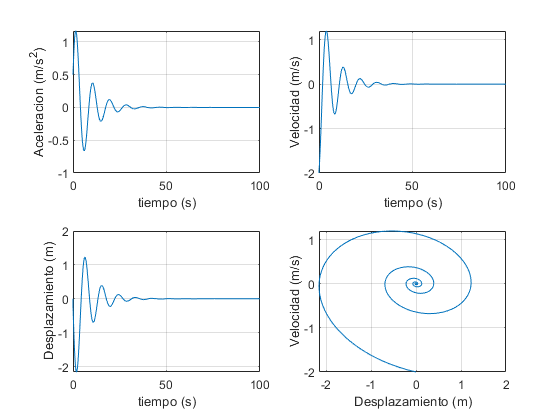
\includegraphics[width=0.9\textwidth]{images/002A.png}
    \caption{$x-t$, $v-t$, $a-t $~y $v-x$}
\end{figure}

\newpage
\clearpage

\begin{figure}[H]
\centering
    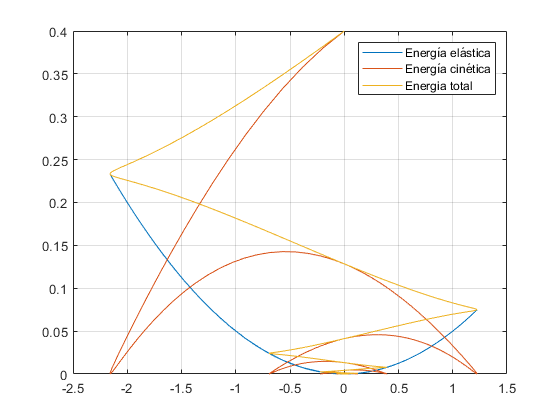
\includegraphics[width=0.5\textwidth]{images/002B1.png}
    \caption{$h=0.1$}
\end{figure}

\begin{figure}[H]
\centering
    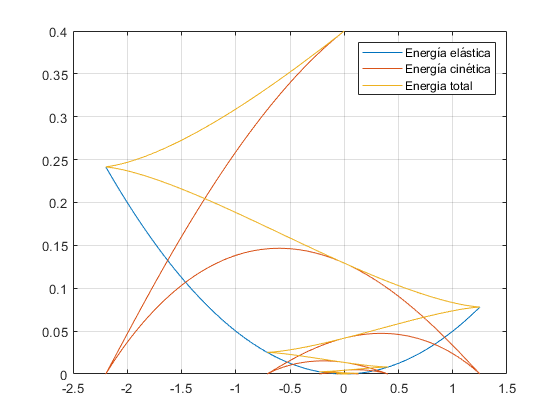
\includegraphics[width=0.5\textwidth]{images/002B2.png}
    \caption{$h=0.01$}
\end{figure}

\begin{figure}[H]
\centering
    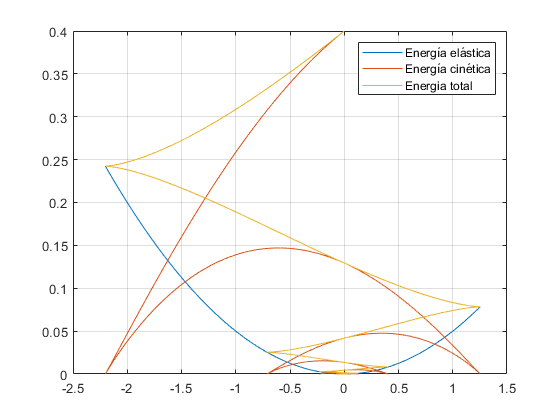
\includegraphics[width=0.5\textwidth]{images/002B3.png}
    \caption{$h=0.001$}
\end{figure}

\clearpage
\newpage

\begin{figure}[H]
\centering
    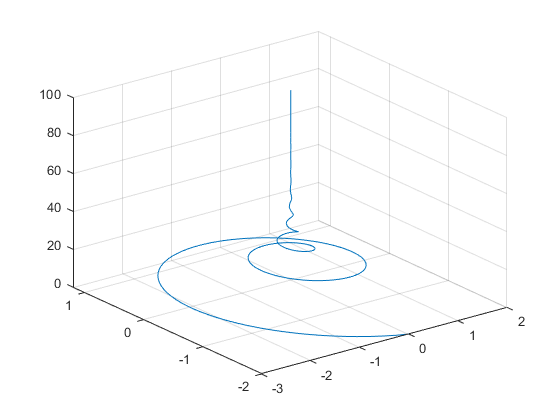
\includegraphics[width=0.7\textwidth]{images/002C.png}
    \caption{$v-x-t$}
\end{figure}


\section{Ejercicio 3}

\begin{lstlisting} [frame=single]
clear; clf; hold off; n=0; h=0.001;
% Constantes del Sistema
k=0.1; m=0.2; c=0.05; F0=0.2; w=0.2;
% Condiciones Iniciales
t=0; x=-1; vx=1; tfin=100; ax=-k*x/m-c*vx/m+F0/m*cos(w*t);
% Inicio de la Simulacion
pt(1)=t; pv(1)=vx; px(1)=x; pa(1)=ax;
pU(1) = 0.5 * k * x ^ 2;
pK(1) = 0.5 * m * vx ^ 2;
pE(1) = pU(1) + pK(1);

for t=0:h:tfin
    n  = n+1;
    ax =-k*x/m-c*vx/m+F0/m*cos(w*t);
    vx = vx + ax*h;
    x  = x  + vx*h;
    U = 0.5 * k * x .^ 2;
    K = 0.5 * m * vx .^ 2;
    E = U + K;
    pt(n+1)=t;
    px(n+1)=x;
    pv(n+1)=vx;
    pa(n+1)=ax;
    pU(n+1)=U;
    pK(n+1)=K;
    pE(n+1)=E;
end

% subplot(2,2,1), plot(pt,pa); grid on;
% xlabel('tiempo (s)');
% ylabel('Aceleracion (m/s^2)')
% subplot(2,2,2), plot(pt,pv); grid on;
% xlabel('tiempo (s)');
% ylabel('Velocidad (m/s)')
% subplot(2,2,3), plot(pt,px); grid on;
% xlabel('tiempo (s)');
% ylabel('Desplazamiento (m)')
% subplot(2,2,4), plot(px,pv); grid on;
% xlabel('Desplazamiento (m)');
% ylabel('Velocidad (m/s)')


% plot(px,pU,'DisplayName','Energía elástica')
% hold on
% plot(px,pK,'DisplayName','Energía cinética')
% plot(px,pE,'DisplayName','Energia total')
% grid on;
% legend

% plot3(px,pv,pt)
% grid on
\end{lstlisting}


\begin{figure}[H]
\centering
    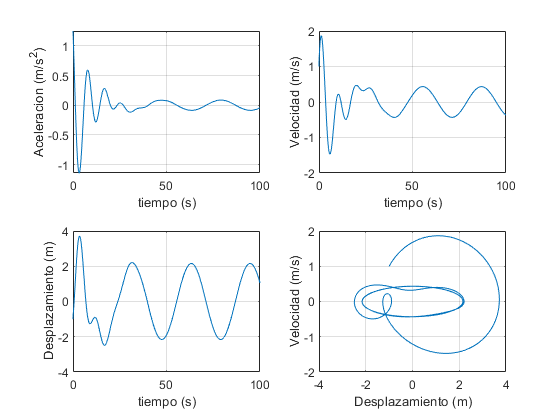
\includegraphics[width=0.9\textwidth]{images/003A.png}
    \caption{$x-t$, $v-t$, $a-t $~y $v-x$}
\end{figure}

\newpage
\clearpage

\begin{figure}[H]
\centering
    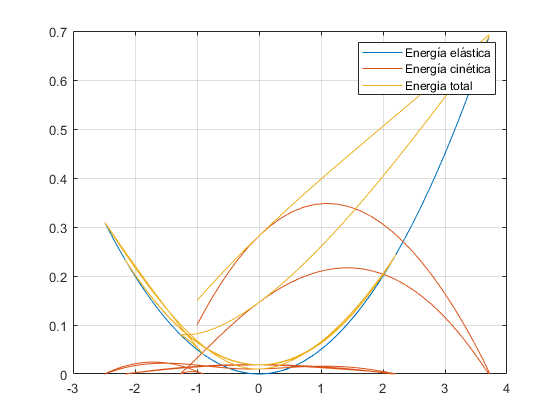
\includegraphics[width=0.5\textwidth]{images/003B1.png}
    \caption{$h=0.1$}
\end{figure}

\begin{figure}[H]
\centering
    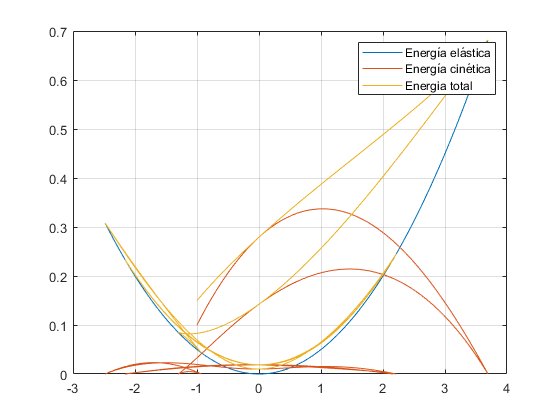
\includegraphics[width=0.5\textwidth]{images/003B2.png}
    \caption{$h=0.01$}
\end{figure}

\begin{figure}[H]
\centering
    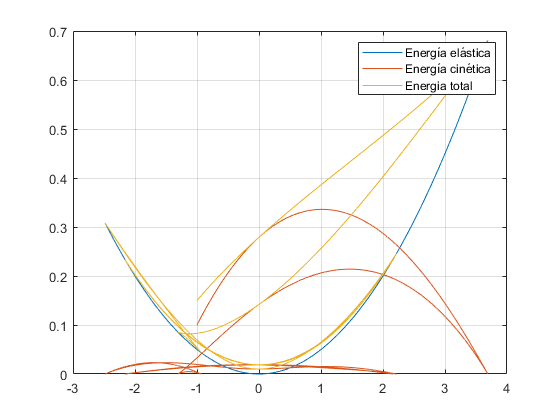
\includegraphics[width=0.5\textwidth]{images/003B3.png}
    \caption{$h=0.001$}
\end{figure}

\clearpage
\newpage

\begin{figure}[H]
\centering
    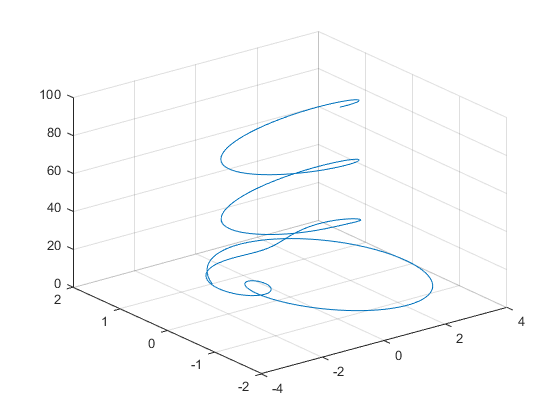
\includegraphics[width=0.7\textwidth]{images/003C.png}
    \caption{$v-x-t$}
\end{figure}

\section{Animaciones}

Enlace a \textcolor{blue}{\href{https://drive.google.com/drive/folders/1uHIAViRx4Gnbq0uHUR8HpsFWhjvJ8CsG?usp=sharing}{GOOGLE DRIVE}} con todos los gifs.

\subsection{Código modificado del ejercicio 1 para los gifs}

\begin{lstlisting} [frame=single]
clear; clf; hold off; n=0; h=0.1;
% Constantes del Sistema
k=0.1; m=0.2; c=0.0; F0=0.0; w=0.0;
% Condiciones Iniciales
t=0; x=2; vx=0; tfin=100; ax=-k*x/m-c*vx/m+F0/m*cos(w*t);
% Inicio de la Simulacion
pt(1)=t; pv(1)=vx; px(1)=x; pa(1)=ax;
pU(1) = 0.5 * k * x ^ 2;
pK(1) = 0.5 * m * vx ^ 2;
pE(1) = pU(1) + pK(1);
drawnow;
frame = getframe(1);
im = frame2im(frame);        
[imind,cm] = rgb2ind(im,256);       
outfile = 'oscilatorioA3.gif';
imwrite(imind,cm,outfile,'gif','DelayTime',0,'loopcount',inf);
for t=0:h:tfin
    n  = n+1;
    ax =-k*x/m-c*vx/m+F0/m*cos(w*t);
    vx = vx + ax*h;
    x  = x  + vx*h;
    U = 0.5 * k * x .^ 2;
    K = 0.5 * m * vx .^ 2;
    E = U + K;
    pt(n+1)=t;
    px(n+1)=x;
    pv(n+1)=vx;
    pa(n+1)=ax;
    pU(n+1)=U;
    pK(n+1)=K;
    pE(n+1)=E;
    drawnow;
    frame = getframe(1);
    im = frame2im(frame);        
    [imind,cm] = rgb2ind(im,256);       
    imwrite(imind,cm,outfile,'gif','DelayTime',0,'writemode','append');
    plot3(px,pv,pt);
end
\end{lstlisting}

\begin{itemize}
    \item Para $h=0.1$ \textcolor{blue}{
    \href{https://drive.google.com/file/d/1WXkhg7N2HJBfWSU8vckPY2pPMvStEJgV/view?usp=sharing}{Gif \#1}}.
    \item Para $h=0.01$ \textcolor{blue}{
    \href{https://drive.google.com/file/d/1vKKF7YbgDsOPVjdOpqd4qbmjKXZh8aB2/view?usp=sharing}{Gif \#2}}.
\end{itemize}

\subsection{Código modificado del ejercicio 2 para los gifs}

\begin{lstlisting} [frame=single]
clear; clf; hold off; n=0; h=0.01;
% Constantes del Sistema
k=0.1; m=0.2; c=0.05; F0=0.0; w=0.0;
% Condiciones Iniciales
t=0; x=0; vx=-2; tfin=100; ax=-k*x/m-c*vx/m+F0/m*cos(w*t);
% Inicio de la Simulacion
pt(1)=t; pv(1)=vx; px(1)=x; pa(1)=ax;
pU(1) = 0.5 * k * x ^ 2;
pK(1) = 0.5 * m * vx ^ 2;
pE(1) = pU(1) + pK(1);
drawnow;
frame = getframe(1);
im = frame2im(frame);        
[imind,cm] = rgb2ind(im,256);       
outfile = 'oscilatorioB2.gif';
imwrite(imind,cm,outfile,'gif','DelayTime',0,'loopcount',inf);
for t=0:h:tfin
    n  = n+1;
    ax =-k*x/m-c*vx/m+F0/m*cos(w*t);
    vx = vx + ax*h;
    x  = x  + vx*h;
    U = 0.5 * k * x .^ 2;
    K = 0.5 * m * vx .^ 2;
    E = U + K;
    pt(n+1)=t;
    px(n+1)=x;
    pv(n+1)=vx;
    pa(n+1)=ax;
    pU(n+1)=U;
    pK(n+1)=K;
    pE(n+1)=E;
    drawnow;
    frame = getframe(1);
    im = frame2im(frame);        
    [imind,cm] = rgb2ind(im,256);       
    imwrite(imind,cm,outfile,'gif','DelayTime',0,'writemode','append');
    grid on
    plot3(px,pv,pt);
end
\end{lstlisting}

\begin{itemize}
    \item Para $h=0.1$ \textcolor{blue}{
    \href{https://drive.google.com/file/d/1vKKF7YbgDsOPVjdOpqd4qbmjKXZh8aB2/view?usp=sharing}{Gif \#3}}.
    \item Para $h=0.01$ \textcolor{blue}{
    \href{https://drive.google.com/file/d/1vKKF7YbgDsOPVjdOpqd4qbmjKXZh8aB2/view?usp=sharing}{Gif \#4}}.
\end{itemize}

\subsection{Código modificado del ejercicio 3 para los gifs}

\begin{lstlisting} [frame=single]
clear; clf; hold off; n=0; h=0.01;
% Constantes del Sistema
k=0.1; m=0.2; c=0.05; F0=0.2; w=0.2;
% Condiciones Iniciales
t=0; x=-1; vx=1; tfin=100; ax=-k*x/m-c*vx/m+F0/m*cos(w*t);
% Inicio de la Simulacion
pt(1)=t; pv(1)=vx; px(1)=x; pa(1)=ax;
pU(1) = 0.5 * k * x ^ 2;
pK(1) = 0.5 * m * vx ^ 2;
pE(1) = pU(1) + pK(1);
drawnow;
frame = getframe(1);
im = frame2im(frame);        
[imind,cm] = rgb2ind(im,256);       
outfile = 'oscilatorioC2.gif';
imwrite(imind,cm,outfile,'gif','DelayTime',0,'loopcount',inf);
for t=0:h:tfin
    n  = n+1;
    ax =-k*x/m-c*vx/m+F0/m*cos(w*t);
    vx = vx + ax*h;
    x  = x  + vx*h;
    U = 0.5 * k * x .^ 2;
    K = 0.5 * m * vx .^ 2;
    E = U + K;
    pt(n+1)=t;
    px(n+1)=x;
    pv(n+1)=vx;
    pa(n+1)=ax;
    pU(n+1)=U;
    pK(n+1)=K;
    pE(n+1)=E;
    drawnow;
    frame = getframe(1);
    im = frame2im(frame);        
    [imind,cm] = rgb2ind(im,256);       
    imwrite(imind,cm,outfile,'gif','DelayTime',0,'writemode','append');
    grid on
    plot3(px,pv,pt);
end
\end{lstlisting}

\begin{itemize}
    \item Para $h=0.1$ \textcolor{blue}{
    \href{https://drive.google.com/file/d/13oQnvO6wZyXtTE092_Jh6Q3d9C0mVOkc/view?usp=sharing}{Gif \#5}}.
    \item Para $h=0.01$ \textcolor{blue}{
    \href{https://drive.google.com/file/d/1RY2LNtwI4kipP80gi7QYkr8RZ0mx84mb/view?usp=sharing}{Gif \#6}}.
\end{itemize}


\end{document}